\documentclass[11pt,a4paper]{article}
\usepackage[utf8]{inputenc}
\usepackage[T2A]{fontenc}
\usepackage[russian]{babel}
\usepackage{cmap} % searchable/copyable Cyrillic
\usepackage{amsmath,amsthm,amssymb,amsfonts,mathtools}
\usepackage{geometry}
\usepackage{enumitem}
\usepackage{bm}
\usepackage{graphicx} % для вставки рисунков PNG/JPG
\usepackage{caption}
\usepackage{float}

% Загружаем hyperref ПОСЛЕДНИМ, чтобы избежать конфликтов
\usepackage{hyperref}

\geometry{margin=1in}

\hypersetup{
  colorlinks=true,
  linkcolor=blue,
  citecolor=blue,
  urlcolor=blue,
  pdftitle={Фазовая намотка, фазовая плоскость и двойное решето},
  pdfauthor={Автор: <впишите имя>},
  pdfsubject={Препринт},
  pdfkeywords={намотка, фазовая развертка, фазовая плоскость, двойное решето, ABC, простые близнецы}
}

% --- Theorem Environments ---
\newtheorem{definition}{Определение}[section]
\newtheorem{lemma}[definition]{Лемма}
\newtheorem{proposition}[definition]{Утверждение}
\newtheorem{remark}[definition]{Замечание}

% --- Shortcuts ---
\newcommand{\Z}{\mathbb{Z}}
\newcommand{\R}{\mathbb{R}}
\newcommand{\rad}{\operatorname{rad}}
\newcommand{\gcdop}{\operatorname{gcd}}
\newcommand{\modm}{\ (\mathrm{mod}\ m)}

\title{\textbf{Фазовая намотка числовой прямой, фазовая плоскость и двойное решето}\\
\large Короткие определения, простые леммы и заготовки рисунков}
\author{Автор: \textit{Горюшкин Сергей Владимирович zz.vexel@gmail.com}}
\date{\today}

\begin{document}
\maketitle

\begin{abstract}
Документ даёт \emph{максимально простое} описание фазовой намотки: как каждое целое число получает координаты \emph{уровень + высота}, как разворачивается цилиндр в плоскость, что такое \emph{минимальный треугольник} формата $A_0+B_0=C_0$, и как формулируется \emph{двойное решето} для $6k\pm1$. Предназначен для вставки готовых рисунков: цилиндр, фазовая плоскость, решето.
\end{abstract}

\tableofcontents

\section{Намотка: как число n получает координаты}\label{sec:coords}
Фиксируем модуль $m\in\Z_{\ge1}$. \textbf{Наматываем} числовую прямую на цилиндр так, что каждые $m$ шагов по оси попадаем на тот же угол.

\begin{definition}[Координаты числа при намотке]\label{def:coords}
Для $n\in\Z$ определим
\begin{align*}
\text{уровень (фаза):}\quad & v(n)\ :=\ n \bmod m\ \in \{0,1,\dots,m-1\},\\
\text{высота (номер витка):}\quad & h(n)\ :=\ \left\lfloor \frac{n}{m}\right\rfloor \in \Z.
\end{align*}
На цилиндре фаза $v$ отображается в угол $\theta=\frac{2\pi}{m}\,v$, а высота $h$ --- в осевую координату. При \emph{развёртке} цилиндра в плоскость точке $n$ сопоставляется пара $(h(n),\,v(n))\in\Z\times\{0,\dots,m-1\}$.
\end{definition}

\begin{remark}
Говорим: \emph{``число $n$ лежит на уровне $v$ и на высоте $h$''}. При увеличении $n$ на $m$ уровень не меняется, а высота растёт на $1$.
\end{remark}

\begin{figure}[H]
\centering
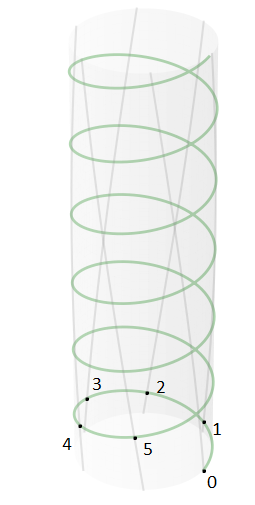
\includegraphics[width=0.4\textwidth]{phase_cylinder.png} % или .jpg
\caption{Фазовая намотка числовой прямой на цилиндр ($m=6$). Числа с одинаковым остатком лежат на одной образующей.}
\label{fig:cylinder}
\end{figure}

\section{Фазовая плоскость (развёртка цилиндра)}
Разворачиваем цилиндр вдоль образующей: получаем \textbf{фазовую плоскость} с прямоугольными координатами $(h,v)$, где $h\in\Z$ (высота) и $v\in\{0,\dots,m-1\}$ (уровень), периодически повторяющийся по $v$ с периодом $m$.

\begin{proposition}[Точка $\to$ прямая уровня]\label{prop:level-lines}
Множество $\{n\in\Z:\ v(n)=r\}$ при развёртке образует горизонтальную прямую уровня $v=r$. Все уровни $v=0,1,\dots,m-1$ --- параллельны.
\end{proposition}

\begin{proposition}[Повороты/степени по фазе]\label{prop:powers}
Если считать фазу как угол $\theta=\frac{2\pi}{m}v$, то операция ``$n$-я степень'' действует по фазе как умножение: $v\mapsto (n\cdot v)\bmod m$. На плоскости это замена уровня $v$ на $n v\mod m$.
\end{proposition}

\begin{figure}[H]
\centering
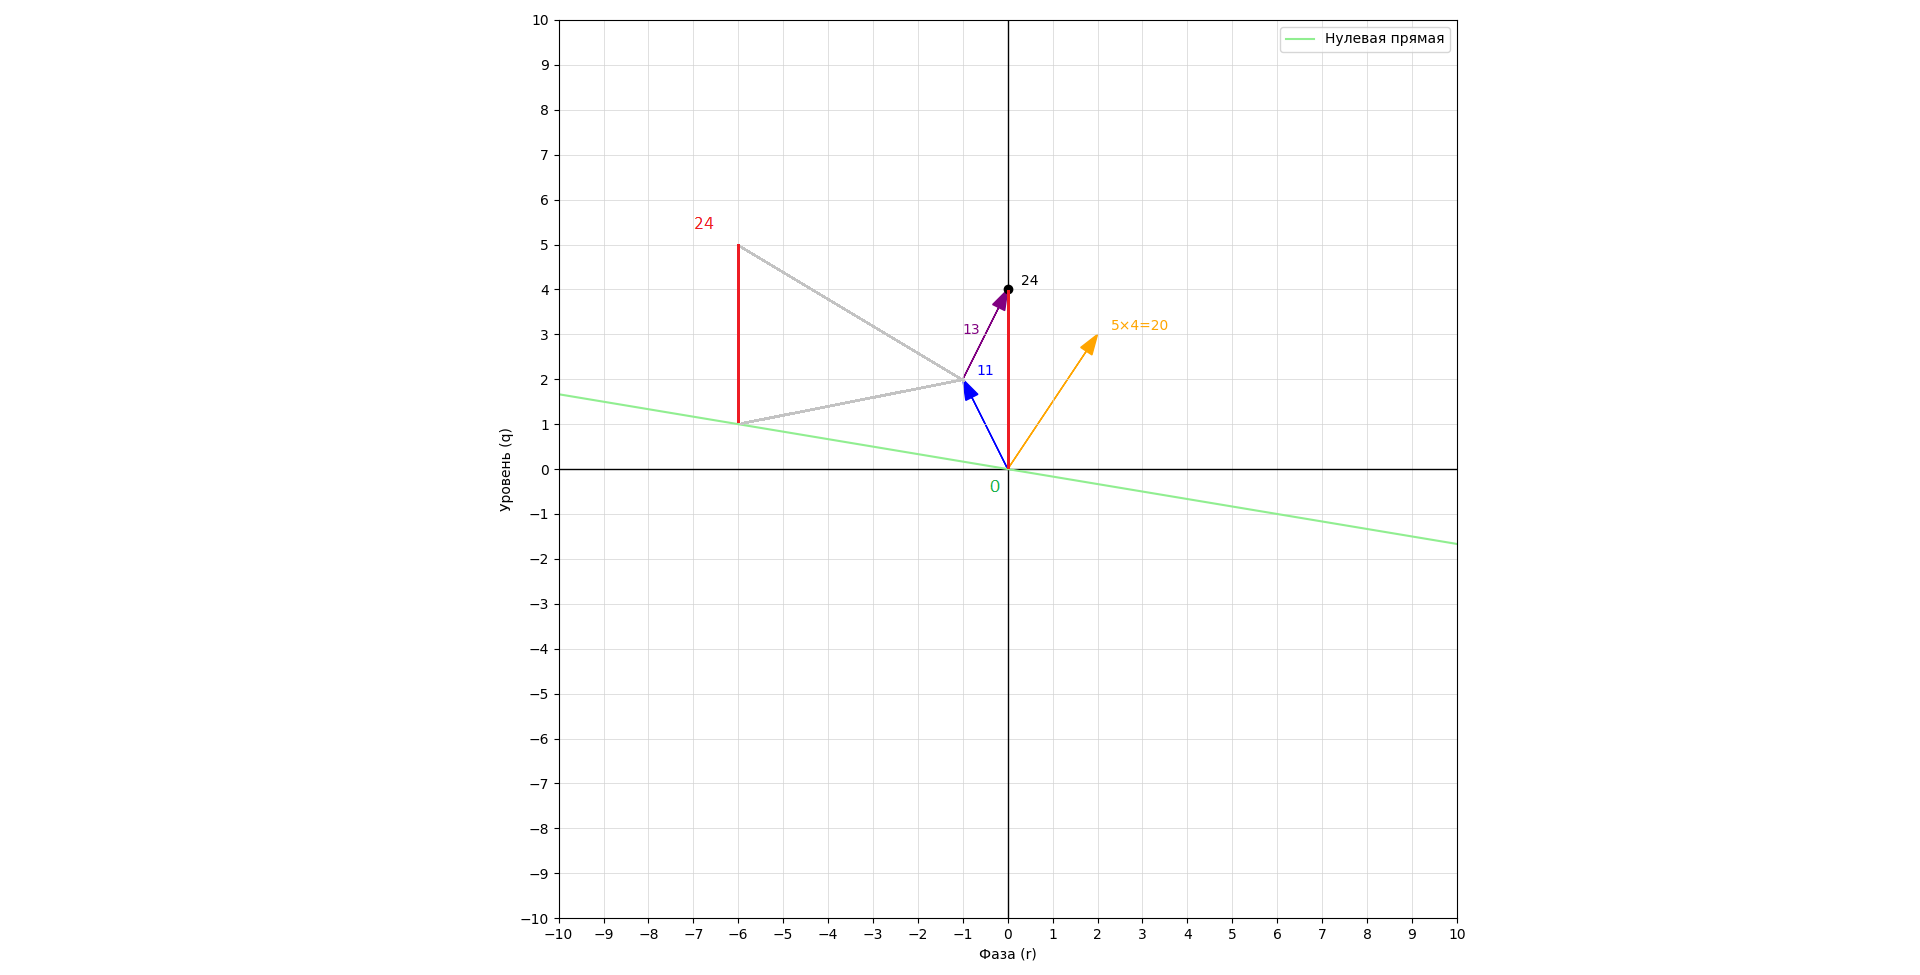
\includegraphics[width=0.9\textwidth]{phase_plane.png} % или .jpg
\caption{Фазовая плоскость: развёртка цилиндра. Горизонтальные линии соответствуют фиксированным фазам (остаткам по модулю $m$).}
\label{fig:plane}
\end{figure}

% --- Минимальный треугольник: якорная версия и эквивалентность ---

\begin{definition}[Минимальный треугольник; якорная версия]
Пусть фиксирован модуль $m\ge1$ и остатки $(A_0,B_0,C_0)\in\{0,\dots,m-1\}^3$
удовлетворяют $A_0+B_0\equiv C_0\pmod m$. 
\emph{Якорным семейством} (с якорем $A$) называем множество решений
\[
\mathcal S_{A_0}\ :=\ \bigl\{(A,B,C):\ A=A_0,\ \ B=B_0+km,\ \ C=C_0+km,\ k\in\mathbb Z\bigr\}.
\]
Интуитивно: $A$ фиксирован как «фазовый якорь», а $(B,C)$ поднимаются синхронно на один виток.
\end{definition}

\begin{lemma}[Эквивалентность с полной решёточной параметризацией]
Полная параметризация решений
\[
A=A_0+mx,\qquad B=B_0+my,\qquad C=C_0+m(x+y)\qquad (x,y\in\mathbb Z)
\]
содержит якорное семейство как срез $x=0,\ y=k$. 
Наоборот, любое решение с $A\equiv A_0\ (\mathrm{mod}\ m)$ можно свести к якорной форме:
выбрав $x$ из равенства $A=A_0+mx$ и положив $k=y$, получаем $(A,B,C)\in\mathcal S_{A_0}$ после вычитания $mx$ из $B$ и $C$.
\end{lemma}

\begin{remark}[Пример при $m=6$]
Для минимального треугольника $(A_0,B_0,C_0)=(1,2,3)$ якорное семейство по $A$:
\[
(1,\ 2+6k,\ 3+6k),\qquad k\in\mathbb Z,
\]
что эквивалентно общей формуле при $x=0,\ y=k$. Аналогично можно якорить $B$ или $C$:
$(A,B,C)=(A_0+km,\ B_0,\ C_0+km)$ или $(A_0+km,\ B_0+km,\ C_0)$.
\end{remark}


\section{Двойное решето для 6k±1}
Фиксируем $z\ge5$, множество простых $\mathcal P(z)=\{p:\ 5\le p\le z\}$, и $M=\prod_{p\in\mathcal P(z)}p$. Для $p\in\mathcal P(z)$ пусть $t_p\equiv 6^{-1}\pmod p$.

\begin{lemma}[Двойное решето]\label{lem:double}
Множество индексов
\begin{equation*}
S(z)=\bigl\{\,k\in\Z:\ \forall p\in\mathcal P(z)\ \ k\not\equiv \pm t_p\ (\bmod p)\,\bigr\}
\end{equation*}
имеет период $M$ и в одном периоде содержит ровно
\begin{equation*}
\varphi_2(M)=\prod_{p\in\mathcal P(z)}(p-2)
\end{equation*}
разрешённых классов. Каждому разрешённому классу $k\equiv r\pmod M$ соответствует \emph{двойная} прогрессия $6(r+jM)\pm1$ без делителей $\le z$.
\end{lemma}

\begin{figure}[H]
\centering
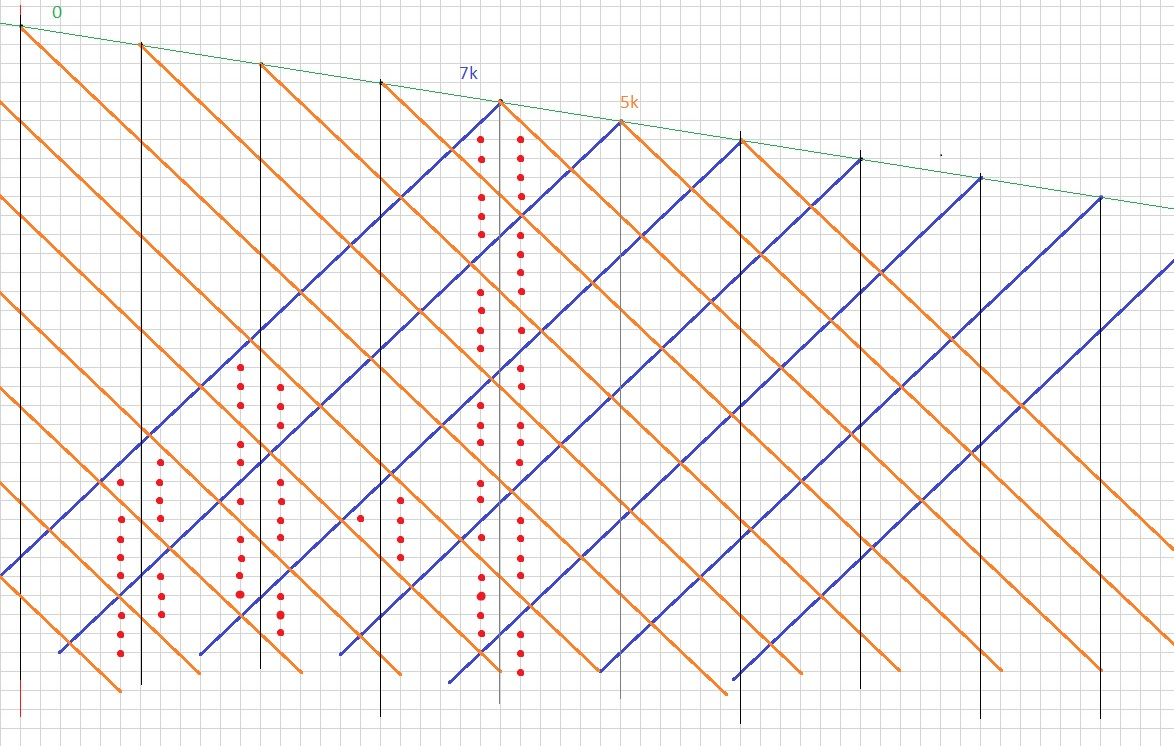
\includegraphics[width=0.9\textwidth]{double_sieve.png} % или .jpg
\caption{Двойное решето для $m=30$. Красные точки показывают вероятного простого.}
\label{fig:sieve}
\end{figure}
\begin{remark}[Пояснение к рисунку двойного решета]
На рисунке изображены два ситовых слоя: 
\begin{itemize}
  \item \textbf{левое решето} $5k$ (запреты по простому $p=5$),
  \item \textbf{правое решето} $7k$ (запреты по простому $p=7$).
\end{itemize}
Они даны в виде наклонных прямых, которые образуют перекрёстную решётку на фазовой плоскости.

Вдоль нулевой оси (вертикаль $6k$) вниз идут каналы $6k\pm1$. 
По обе стороны от неё нанесены красные точки~--- кандидаты на простые. 
До момента пересечения $5\cdot 7=35$ все эти точки являются потенциально простыми:
\[
11,\ 13,\ 17,\ 19,\ 23,\ 29, \dots
\]
Некоторые из них будут выбиваться последующими решётами (по большим простым).

Характерные места:
\begin{itemize}
  \item на левом канале (через $v=5$) видно последовательность $11,13,19,\dots$, но в точке $25$ срабатывает решето $5k$;
  \item на правом канале (через $v=1$) идут $11,17,23,29$, а затем в точке $35$ срабатывает \emph{двойное пересечение} решёт $5k$ и $7k$.
\end{itemize}

Таким образом рисунок демонстрирует: \emph{каждый красный маркер --- это «живое место» ситовой решётки, пока его не исключит одно из следующих простых.}
\end{remark}
\section{Гипотеза щита}

\paragraph{Определение (щитового окна).}
Пусть \(p<q\) --- \emph{соседние простые числа}. Определим \emph{щитовым окном} интервал
\[
W(p)\ :=\ \bigl(p^2,\ q^2\bigr).
\]
Внутри \(W(p)\) сито на каналах \(6k\pm1\) действует только ограничениями от простых \(\le p\);
следующий простой \(q\) «включается» лишь на правой границе \(q^2\).

\paragraph{Наблюдение (пример \(p=5,\ q=7\)).}
В окне \(W(5)=(25,49)\) на каналах \(6k\pm1\) остаются простые
\[
29,\ 31,\ 37,\ 41,\ 43,\ 47,
\]
в частности появляется \emph{пара близнецов} \(29,31\).
Здесь новые ситовые ограничения начинают работать только с числа \(49=7^2\).

\paragraph{Формулировка (гипотеза щита).}
Если в некотором щитовом окне \(W(p)=(p^2,q^2)\) существует пара близнецов \((u,u+2)\),
то пары близнецов существуют и в бесконечно многих последующих окнах \(W(p')\) при \(p'\to\infty\).

\paragraph{Индуктивная эвристика.}
Структура запретов в \(W(p)\) описывается периодом
\[
M(p)=\prod_{\,5\le r\le p} r
\]
по китайской теореме об остатках.
Наличие пары близнецов означает, что в этом слове из «живых» и «дыр» есть два соседних разрешённых места.
При переходе к следующему окну \(W(p')\) этот шаблон поднимается по модулю \(M(p)\) (и его расширениям).
Таким образом, \emph{если пара близнецов появилась в одном щитовом окне, то по индукции она будет появляться и в последующих окнах}, сохраняясь в бесконечной последовательности.

\section{Провал радикала: что это и как он ограничен}
\newcommand{\isanchorA}{\text{(якорим $A$;\ $x=0$,\ $B=B_0+my,\ C=C_0+my$)}} % краткая помета
% --- Провал радикала: два режима и "коэффициент качества" ---
\begin{lemma}[Провал радикала: общий vs якорный режим]
Пусть $m\ge1$, $A_0+B_0\equiv C_0\ (\mathrm{mod}\ m)$ и
\[
A=A_0+mx,\quad B=B_0+my,\quad C=C_0+m(x+y).
\]
Обозначим $C_0'=\rad\!\big(\gcd(A_0,B_0)\gcd(A_0,C_0)\gcd(B_0,C_0)\big)$ и $C_m=\rad(m)$. Тогда
\[
\Delta(A,B,C)=\frac{\rad(A)\rad(B)\rad(C)}{\rad(ABC)}\le
\begin{cases}
C_0'\,C_m^{\,2}, & \textbf{общий случай},\\[2mm]
C_0'\,C_m, & \textbf{якорный режим }\isanchorA.
\end{cases}
\]
\end{lemma}

\begin{remark}[Уточнение якорного режима]
В якорном режиме вклад простых $p\mid m$ зависит только от остатков $A_0,B_0,C_0$.
Если дополнительно $\gcd(A_0,m)=1$, то для всех $p\mid m$ имеем $k_p\le1$ и
\[
\Delta(A,B,C)\le C_0'. 
\]
Вообще всегда справедлива более тонкая оценка
\[
\Delta(A,B,C)\ \le\ C_0'\,\rad\!\big(\gcd(A_0,m)\big),
\]
а грубая линейная $C_0' C_m$ удобна как универсальная «короткая» граница.
\end{remark}

\begin{remark}[Коэффициент качества]
Введём \emph{коэффициент качества} класса
\[
\kappa_{\mathrm{gen}}(m):=\rad(m)^{2},\qquad 
\kappa_{\mathrm{anc}}(A_0;m):=\rad(m)\quad\text{(или тоньше }\rad(\gcd(A_0,m))\text{)}.
\]
Тогда $\Delta\le C_0'\,\kappa$, и чем меньше $\kappa$, тем «чище» тройка по смыслу ABC:
якорение и взаимная простота $A_0$ с $m$ минимизируют провал радикала.
\end{remark}


\begin{proof}[Идея доказательства]
Пусть $k_p$ — число из $\{0,1,2,3\}$, равное количеству компонент $A,B,C$, делящихся на простой $p$.
Тогда вклад $p$ в $\Delta$ равен $p^{k_p-1}$, откуда общий верхний предел $k_p-1\le2$ даёт $\rad(m)^2$.
В якорном случае из $A_0+B_0\equiv C_0\ (\bmod p)$:
если $p\nmid A_0$, то $B_0$ и $C_0$ не могут одновременно делиться на $p$ ($k_p\le1$);
если $p\mid A_0$ и класс минимален (не все три делятся на $p$), то $k_p\le2$, что даёт множитель не выше $p$.
Если кроме того $\gcd(A_0,m)=1$, то для всех $p\mid m$ имеем $k_p\le1$ и вклад равен $1$.
\end{proof}
\begin{figure}[H]
  \centering
  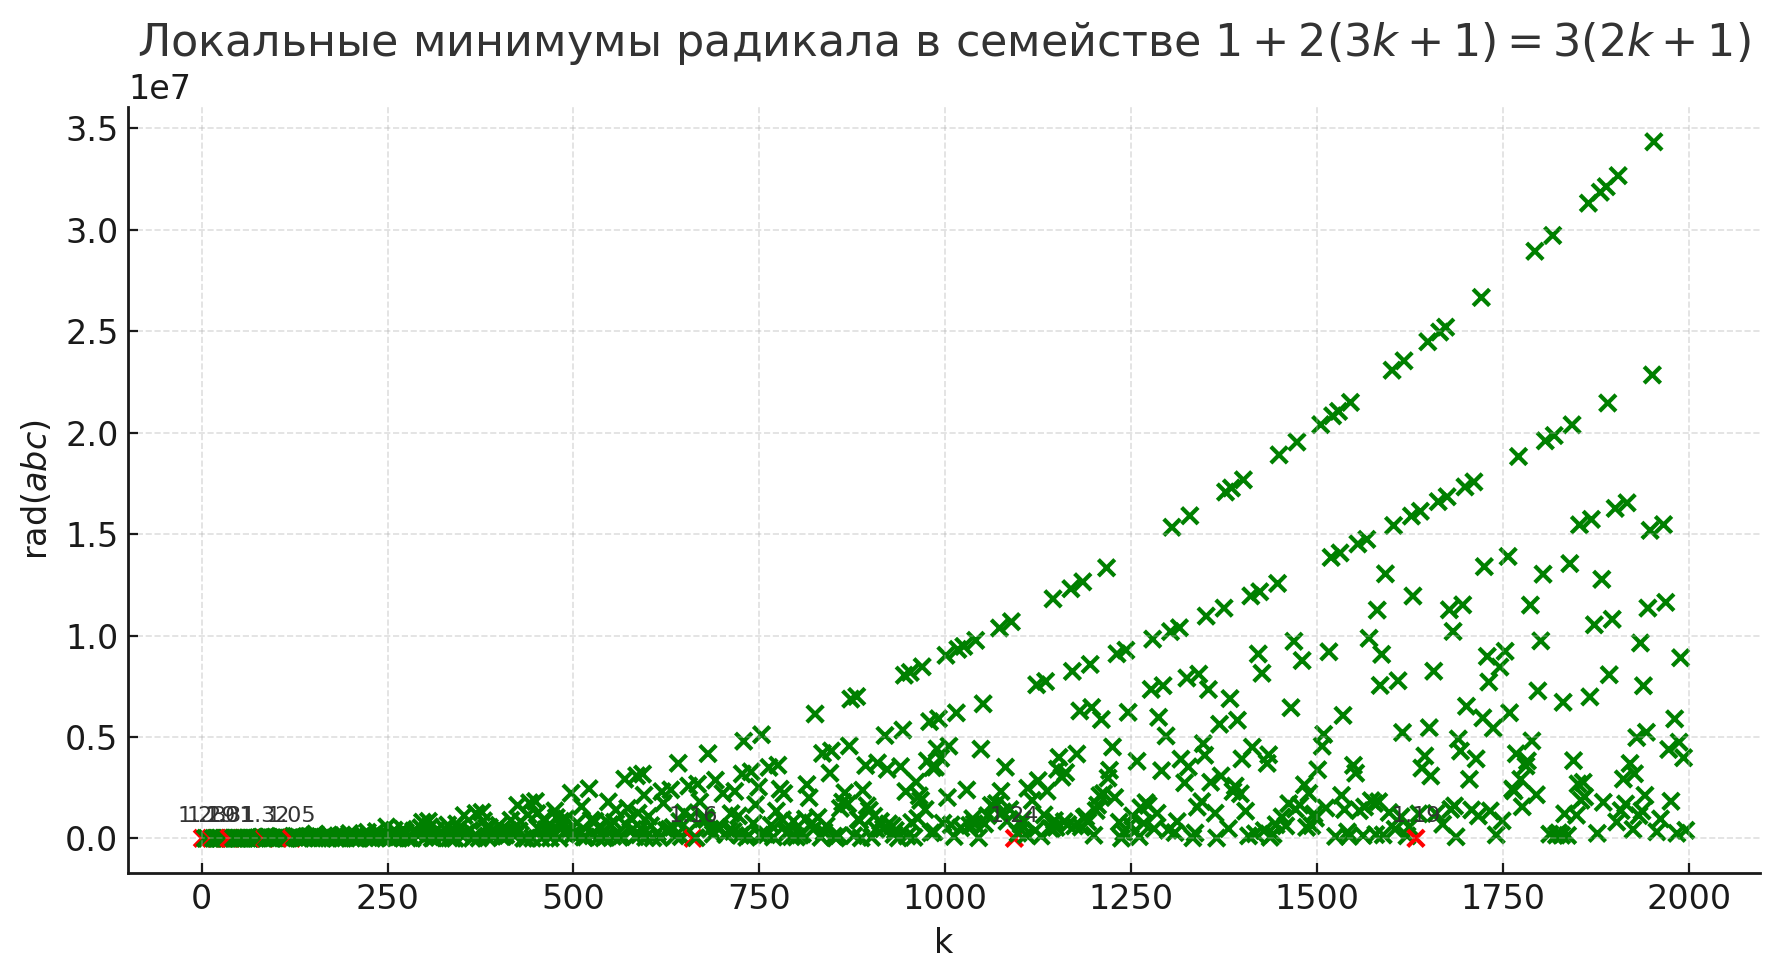
\includegraphics[width=0.92\linewidth]{rad-fall-graph.png} % <-- положи файл, напр. rad-fall-graph.pdf/png
  \caption{Провал радикала \(\Delta\) в якорном режиме: $A=A_0$ фиксирован, 
  $(B,C)=(B_0+my,\ C_0+my)$. Резкие падения соответствуют появлению общего простого делителя,
  границы сверху соответствуют оценкам из леммы (\(C_0'\,C_m\) или тоньше \(C_0'\rad(\gcd(A_0,m))\)).}
  \label{fig:rad-fall-graph}
\end{figure}
\begin{remark}[Геометрия провала на графике]
В якорном режиме $A$ фиксирован, а $(B,C)=(B_0+my,\ C_0+my)$ сдвигаются синхронно.
Поэтому соседние точки $y$ дают почти совпадающие величины $B$ и $C$ (различаются на шаг $m$),
а при попадании общего простого делителя в обе компоненты радикал $\rad(ABC)$ резко ``схлопывается'',
что видно как скачок вниз у $\Delta$ на графике (\emph{провал}).
\end{remark}

% ===== TOR: двухфазная намотка и КТО =====
\section{TOR: двухфазная намотка и китайская теорема об остатках}

\begin{definition}[Двухфазная намотка и тор]
Пусть $m_1,m_2\in\mathbb Z_{\ge1}$. Для $n\in\mathbb Z$ зададим две фазы
\[
v_1(n):=n\bmod m_1,\qquad v_2(n):=n\bmod m_2.
\]
Отображение
\[
\Phi:\ \mathbb Z\to (\mathbb Z/m_1\mathbb Z)\times(\mathbb Z/m_2\mathbb Z),\qquad
\Phi(n)=(v_1(n),v_2(n))
\]
— это двухфазная намотка на тор $S^1\times S^1$ (комбинаторно — прямоугольная решётка остатков).
\end{definition}

\begin{proposition}[Аналог КТО на торе]
Если $\gcd(m_1,m_2)=1$, то для любых остатков $a\ (\bmod m_1)$, $b\ (\bmod m_2)$ существует единственный
класс $n\ (\bmod M)$, $M=m_1m_2$, такой что
\[
n\equiv a\pmod{m_1},\qquad n\equiv b\pmod{m_2}.
\]
Эквивалентно: орбита $\{\Phi(n):n\in\mathbb Z\}$ проходит по всем клеткам решётки ровно один раз за период $M$.
Если $g=\gcd(m_1,m_2)>1$, орбита распадается на $g$ циклов длины $M/g$.
\end{proposition}

\begin{remark}[Длинная развёртка (идея)]
Разворачивая тор в прямоугольник $[0,m_1)\times[0,m_2)$, траектория $n\mapsto (v_1(n),v_2(n))$
визуализируется как прямая с рациональным наклоном, замыкающаяся с периодом $M$.
Это геометрическая форма китайской теоремы об остатках.
\end{remark}

\begin{remark}[Эллиптическая кривая на торе (набросок)]
Наложив алгебраическое условие (например, $y^2=x^3+Ax+B$ на одной фазе) и сочетая его с второй фазой,
получаем кривую на торе с выделенной «центральной» точкой — геометрическим образом точки на бесконечности.
Этот пункт даёт направление для дальнейшего анализа и визуализаций.
\end{remark}

% --- один рисунок тора без нумерации и ссылок ---
\begin{center}
  % положите файл в images/ или рядом с .tex; разрешены .pdf/.png/.jpg
  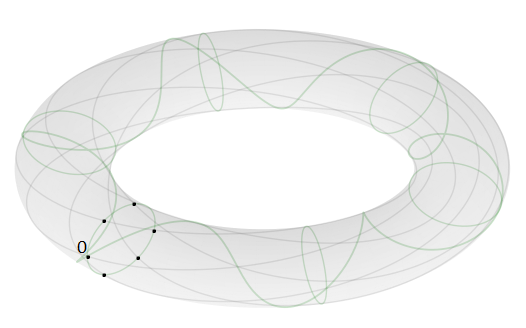
\includegraphics[width=0.85\linewidth]{torus}
\end{center}


\section*{Заключение}

В работе построена геометрическая интерпретация числовой прямой через намотку на цилиндр
и фазовую развёртку. Мы выделили минимальные треугольники как базовые шаблоны для троек $A+B=C$,
а также показали, что операции сдвига и подъёма согласуются с векторными операциями на фазовой плоскости.

Далее введена \emph{гипотеза щита}: в каждом окне $(p^2,(p+1)^2)$ для соседних простых $p<p+1$
остаётся ненулевая конфигурация кандидатов на простые, и наличие пары близнецов в одном окне
эвристически гарантирует их повторение в последующих окнах.

Мы уточнили понятие \emph{провала радикала}: в общем случае он ограничен $C_0'\,\rad(m)^{2}$,
а в якорном режиме — $C_0'\,\rad(m)$, что даёт простую эвристику оценки качества троек $(A,B,C)$
в терминах гипотезы ABC.

Наконец, введён \emph{тор} как геометрический аналог китайской теоремы об остатках:
двухфазная намотка $n\mapsto (n\bmod m_1,\,n\bmod m_2)$ реализует структуру CRT на поверхности $S^1\times S^1$.
Это открывает путь к дальнейшим конструкциям (в частности, к эллиптическим кривым на торе).

Таким образом, добавленные фрагменты (щит, провал радикала, тор) формируют целостную картину:
геометрическая интерпретация даёт не только наглядность, но и комбинаторные эвристики
для классических задач теории чисел.



\bigskip
\noindent\textbf{Контакты автора:} \texttt{zz.vexel@gmail.com/ GitHub zzVex }.

\end{document}